\documentclass[twocolumn]{IEEEtran}

\IEEEoverridecommandlockouts
% The preceding line is only needed to identify funding in the first footnote. If that is unneeded, please comment it out.
\usepackage{cite}
\usepackage{amsmath,amssymb,amsfonts,amsthm}
\usepackage{algorithmic}
\usepackage{graphicx}
\usepackage{textcomp}
\usepackage{xcolor}

\ifCLASSOPTIONcompsoc
\usepackage[caption=false, font=normalsize, labelfont=sf, textfont=sf]{subfig}
\else
\usepackage[caption=false, font=footnotesize]{subfig}
\fi

\newtheorem{lemma}{Lemma}
\renewcommand{\IEEEQED}{\IEEEQEDclosed}

\def\BibTeX{{\rm B\kern-.05em{\sc i\kern-.025em b}\kern-.08em
    T\kern-.1667em\lower.7ex\hbox{E}\kern-.125emX}}

\begin{document}
\section*{Introduction}
The aim of this section is to explain in detail the data flow and the stages during the finding of flocks following a distributed approach.  In general, we can break down the process as follows:
\begin{enumerate}
\item Pair finding.
\item Center computation.
\item Disk finding.
\end{enumerate}

The main purpose will be to partition the space from the very beginning and ensure all the required data is accessible to each partition.  We expect to exploit locality at most and minimize the impact of any required shuffling.   


\subsection*{Pair finding}
We start dividing the input point-set into partitions using a quadtree data structure.  Each leaf in the quadtree will be used as a partition which divides the point-set into no overlapping areas.  We will call the space covered by an individual leaf as a \textit{cell}.

It is important to note that a point close to the border of a cell could be matched with points laying in contiguous cells.  So, it is required to replicate the data around each cell to deal with those cases.  Each cell will have an expansion zone which width is equal to $\varepsilon$ (the distance required between points to be consider a pair). In Fig. \ref{fig:inputa} the expansion zone is described by the red dotted lines around each cell.  Similarly, Fig. \ref{fig:inputb} shows how the points in the expansion zone are replicated to the involved cells.  It is expected that each cell is evaluated by different nodes safely as each one has the required data.

\begin{figure}[htbp]
  \centering
  \subfloat[Input point-set\label{fig:inputa}]{%
    \includegraphics[page=4, width=1\columnwidth]{figures/lema1}
  }
  \\
  \subfloat[Partitions with replicated data\label{fig:inputb}]{%
    \includegraphics[page=5, width=1\columnwidth]{figures/lema1}
  }
  \caption{Partitioning and replication.}
  \label{fig:input}
\end{figure}

The pair finding takes place at each cell.  We perform a partition-based self-distance join using  $\varepsilon$ as the distance parameter.  A simple distance-join will generate duplicate pairs (point A matches point B and point B matches A) so we filter them using the point's id. Pairs were point B's id is greater than point A's id are pruned. 

\subsection*{Center computation}
From each pair (formed by points A and B), two circles with radius $\frac{\varepsilon}{2}$ will be computed.  These two circles have points A and B on their circumference. We will show that if the position of a circle's center lies inside of the current cell they will be safe to operate but those located in the expansion zone or outside of it will require special attention.  

Circles with centers in the expansion zone will be repeated in contiguous cells and will increase the computation cost of further stages.  In addition, it is possible that pairs of points generates circles with centers outside of the expansion zone.  For example, Fig. \ref{fig:centers} illustrates the case.  Circles $a^\prime$ and $b^\prime$ are generated for pairs of points in cells 1 and 2 respectively, however both are located outside of their expansion zone boundaries.  Those circles will be unable to query elements from the original point-set because they were not replicated outside of the expansion zone.  We present lemma \ref{lemma:circles} to show that we can safely remove those kind of circles.

\begin{lemma}\label{lemma:circles}
Circles with its center lying in the expansion zone or outside of it can be discarded as they will be correctly evaluated by one of the cell in its neighborhood. 
\end{lemma}

\begin{proof}
  In order to support our proof we will define some concepts.  First, we will divide the area in three zones to clarify our assumptions:  we already talked about the expansion zone as the area beyond the border of a cell (between black line and dotted red line in Fig. \ref{fig:centers}) and a width equal to $\varepsilon$.  The border zone is a strip of width equal to $\varepsilon$ touching the interior border of a cell.  In Fig. \ref{fig:centers} it is compromised by the dotted blue and the black lines.  The safe zone will be the remaining internal area in the cell which is not covered by the border zone.  Second, we will call the contiguous cell with which the current one will replicate a particular circle as the \textit{replicated cell}. In Fig. \ref{fig:centers}, the cell 2 is the replicated cell of cell 1 and vice versa.

  From here, it will be clear that there is a symmetric relation between the circles in a particular zone in the current cell and the circles in its replicated cell.  We can certainly said that if circle is located in the border zone of the current cell, it will be located in the expansion zone of its replicated cell.  Similarly, any circle with a center lying outside of the expansion zone of the current cell will be located in the safe zone of its replicated cell.  Keeping just the circles with centers lying in the current cell (border or safe zone) will be enough to ensure no lost of information (Fig. \ref{fig:centerspruning}).
\end{proof}

\begin{figure}[htbp]
  \centering
  \includegraphics[page=7, width=1\columnwidth]{figures/lema1}
  \caption{Center computation.}
  \label{fig:centers}
\end{figure}

\begin{figure}[htbp]
  \centering
    \includegraphics[page=8, width=1\columnwidth]{figures/lema1}
  \caption{Center pruning.}
  \label{fig:centerspruning}
\end{figure}

\subsection*{Disk finding}
We call \textit{disk} to the circles (and companion center) together to those points which are enclosed by its circumference.  After the centers computation, this procedure requires to query the points enclosed by the circles of radius $\frac{\varepsilon}{2}$ recently discovered.  We will keep advantage on the current partitioning strategy to perform a partition-based distance join between the set of circles and points.  It is valid to note that no all the points from the original input are needed for this operation.  Lemma \ref{lemma:points} shows that just the points resulting from the pair finding stage are required.  It is important because in order to keep the same partitioning just the points involved during the pair finding remain accessible in the current cell.

\begin{lemma}\label{lemma:points}
Points which are not part of the pair-set are not involved in the disk finding procedure.
\end{lemma}

\begin{proof}
  Let have a point $p_c$ lying inside of a particular circle. So $p_c$ must be located at most $\frac{\varepsilon}{2}$ distance from the center of that circle and, at most, $\varepsilon$ distance to the points $p_a$ and $p_b$ which generated that center.  That means that the $p_c$ itself must form pairs between itself and points $p_a$ and $p_b$ and, therefore, be part of the pair-set.  On the other hand, if a point lies more than $\varepsilon$ distance of any other point, it will not be part of the pair-set and none center will be computed in its surrounding, therefore, it cannot be part of any disk. 
\end{proof}

\end{document}
